%---------------------------------------------------------------------------
%
%                          Vorlage der Arbeitsgruppe
%             Computer Vision and Pattern Recognition Group (CVPR)
%                           der Universität Münster
%                         http://cvpr.uni-muenster.de
%
%---------------------------------------------------------------------------
% Geeignet für:
%  - Seminararbeiten
%  - Bachelorarbeiten
%  - Masterarbeiten
%---------------------------------------------------------------------------
% Autoren:
%  - Daniel Tenbrinck
%  - Fabian Gigengack
%  - Michael Schmeing
%  - Lucas Franek
%  - Andreas Nienkötter
%---------------------------------------------------------------------------
% Version:
%  - 1.0.3 (05.10.2016)
%	 - Ersetzung von veralteten Befehlen durch Aktuelle
%	 - Einige ausführlichere Beispiele
%    - Einführung von listings
%    - Aktuelle Version der Eidesstattlichen Erklärung
%  - 1.0.2 (09.09.2011)
%    - Titelblatt um Matrikelnummer und Studiengang ergänzt
%  - 1.0.1 (05.07.2011)
%---------------------------------------------------------------------------
% 
% "THE BEER-WARE LICENSE" (Revision 42):
% The above mentioned authors wrote this file. As long as you retain this
% notice you can do whatever you want with this stuff. If we meet some day,
% and you think this stuff is worth it, you can buy us a beer in return.
%  --------------------------------------------------------------------------

\documentclass[a4paper, oneside,openany, 12pt, ngerman, listof=nochaptergap, bibliography=totoc,
,listof=totoc,listof=entryprefix,]{scrbook} % Layout-Einstellungen für das Dokument
%openany -> keine leeren Seiten nach chapter

\usepackage[utf8]{inputenc} % UTF-8 Codierung
\usepackage[ngerman]{babel} % Deutsche Beschriftung

\usepackage{graphicx} % Um Bilder einzufügen
%\usepackage{subfigure} % Um mehrere Bilder in eine figure einzufügen

\usepackage{verbatim} % Um Quellcode in das Dokument einzufügen.
\usepackage{xcolor} % Für Farben
\usepackage[linkbordercolor=blue]{hyperref} % Für Links im Dokument
%\usepackage[colorlinks = true,linkcolor = black,urlcolor  = blue,anchorcolor = blue]{hyperref}
            
            
\usepackage{algorithmic} % Für Pseudo-Code
\usepackage{algorithm} % Wrapper für Pseudo-Code
\usepackage[linkbordercolor=blue]{hyperref} % Für Links im Dokument
\usepackage[font={small}, labelfont=bf]{caption} % kleine Bildunterschriften
%\setlength{\abovecaptionskip}{1pc}  % 1pc=12pt
%\setlength{\belowcaptionskip}{1pc}
\usepackage{subcaption}


\usepackage{wrapfig}


\usepackage{geometry} % Für Feinanpassungen des Layouts

\usepackage{listings} % Für Code-Listings
\renewcommand{\lstlistingname}{Quelltext} %Ändert die Überschrift von Listing nach Quelltext

%Ergänzungen
\usepackage{todonotes}

\usepackage{comment}
\usepackage{amsthm}

% Einstellungen für Abstand an den Rändern
\geometry{a4paper,left=35mm,right=35mm,top=20mm,bottom=20mm, includeheadfoot}

%Abkürzungen
\usepackage{acronym}


% Folder structure
\usepackage[edges]{forest}
\definecolor{folderbg}{RGB}{124,166,198}
\definecolor{folderborder}{RGB}{110,144,169}
\newlength\Size
\setlength\Size{4pt}
\tikzset{%
  folder/.pic={%
    \filldraw [draw=folderborder, top color=folderbg!50, bottom color=folderbg] (-1.05*\Size,0.2\Size+5pt) rectangle ++(.75*\Size,-0.2\Size-5pt);
    \filldraw [draw=folderborder, top color=folderbg!50, bottom color=folderbg] (-1.15*\Size,-\Size) rectangle (1.15*\Size,\Size);
  },
  file/.pic={%
    \filldraw [draw=folderborder, top color=folderbg!5, bottom color=folderbg!10] (-\Size,.4*\Size+5pt) coordinate (a) |- (\Size,-1.2*\Size) coordinate (b) -- ++(0,1.6*\Size) coordinate (c) -- ++(-5pt,5pt) coordinate (d) -- cycle (d) |- (c) ;
  },
}
\forestset{%
  declare autowrapped toks={pic me}{},
  pic dir tree/.style={%
    for tree={%
      folder,
      font=\ttfamily,
      grow'=0,
    },
    before typesetting nodes={%
      for tree={%
        edge label+/.option={pic me},
      },
    },
  },
  pic me set/.code n args=2{%
    \forestset{%
      #1/.style={%
        inner xsep=2\Size,
        pic me={pic {#2}},
      }
    }
  },
  pic me set={directory}{folder},
  pic me set={file}{file},
}


%Verzeichnisse in Inhaltsverzeichnis
%\usepackage[nottoc]{tocbibind}

%Zähler abbildungen
\usepackage{chngcntr}
\counterwithout{figure}{chapter}

\usepackage{multicol}


\usepackage[titletoc]{appendix}
\usepackage{titlesec}


\usepackage{enumitem} 
\setitemize{leftmargin=*}

\renewcaptionname{ngerman}{\figurename}{Abb.}


\usepackage[strings]{underscore}
\newenvironment{abstract}{%
  \begin{center}\normalfont\usekomafont{disposition}Abstract\end{center}%
}{%
  \par
  \vfil\null% X
  \endtitlepage% X
}

\usepackage{tikz}%Automaten zeichnen
\usetikzlibrary{positioning,automata,trees,decorations.markings,arrows}

\begin{document}
%Einrückungen verhindern
\setlength{\parindent}{0em} 


% Titelblatt
\begin{titlepage}

\begin{centering}
\vspace{4cm}
%\vspace*{\fill}

\includegraphics[width=12cm]{./img/wwu-logo-neu.pdf}

\vspace{2cm} 

{\large
	Praktikum Copmuter Vision\\[0.5cm]
	bei Jun.-Prof. Dr. Benjamin Risse\\[1cm]
}

{\LARGE
	\textbf{Smart Camera Operator}\\[2cm]
}


{\large
	Vorgelegt von:\\[0.5cm]
}



\begin{minipage}{\textwidth}
\begin{minipage}[c]{0.3\textwidth}
\centering
 \begin{tabular}{ll}
 		Tobias Johanning \\
    	{421503} \\
    	{t_joha02@wwu.de} \\
    	 M.Sc. Informatik\\
    \end{tabular}\\
\end{minipage}\hfill
\begin{minipage}[c]{0.3\textwidth}
\centering
   \begin{tabular}{ll}
 		Markus Konetzny \\
    	{406462} \\
    	{m_kone06@wwu.de} \\
    	M.Sc. Informatik\\
    \end{tabular}\\
\end{minipage}\hfill
\begin{minipage}[c]{0.3\textwidth}
\centering
   \begin{tabular}{ll}
 		Tabea Preusser \\
    	{428026} \\
    	{t_preu04@wwu.de} \\
    	M.Sc. Informatik\\
    \end{tabular}\\
\end{minipage}\hfill
\end{minipage}

\vspace{2 cm}
{\large
	Münster, den 05.03.2020\\[1cm]
}
\end{centering}

\vfill


 


\end{titlepage}
\pagenumbering{roman}

% Inhaltsverzeichnis
\tableofcontents

\cleardoublepage


\newpage


\pagenumbering{arabic}
\mainmatter
% Die Hauptkapitel der Arbeit
\chapter{Einleitung}


\section{Motivation}

Im Rahmen eines Projektes des Unternehmens Rimondo sollte ermöglicht werden, dass die Abdeckung der Videoaufnahme von Reitsportturniere maximiert werden soll. Dazu sollen neben den internationalen auch von möglichst vielen, im besten Falle sogar allen, nationalen Turnieren in NRW Videoaufnahmen erstellt werden können, was später auch auf ganz Deutschland erweitert werden soll. Neben Bereitstellung der Turnieraufnahmen in der Mediathek von Rimondo sind auch Live-Aufnahmen in der Zukunft geplant. Alleine 2018 fanden in NRW über 600 nationale und 82 internationale Reitsportturniere statt, von denen nur ein Bruchteil verfilmt wurde.
Dabei stellt das grundlegende Problem die hohen Personalkosten der Kameraleute dar, die für stundenlange professionelle Aufnahmen benötigt werden. Während dies für internationale Turniere, wie das „Turnier der Sieger“ in Münster, möglich über Fernsehsender zu finanzieren ist, sind die Kosten für die kleineren, regionalen Turniere nicht rentabel. Da jedoch die Kundengruppe, welche aus den Turnierteilnehmern und deren Fans besteht, mit über 98.000 Mitgliedern in Reitsportvereinen in NRW als mögliche Kunden, großes Potenzial darstellt, wird eine Lösung benötigt. Aus diesem Grund wurden Projektgruppen von Informatikstudenten der WWU vor die Aufgabe gestellt die Kameraführung für Reitsportturniere zu automatisiert, indem ein „Smart Camera Operator“ im Rahmen eines Praktikums erstellt wird. Dies sollte eine Software umfassen, welche in der Lage ist den Kameramann für Turnieraufnahmen im Pferdesport zu ersetzen.



\section{Aufgabenstellung und Zielsetzung}

Die Erstellung des „Smart Camera Operators“ zur Videoaufnahme von Reitsportturnieren sollte in drei Phasen unterteilt erreicht werden, wobei die Wahl der Methoden und Verfahren freigestellt wurde.

Die erste Phase hatte die Erstellung von Trainingsdaten von Pferden und Reitern zum Ziel, womit die Vorarbeit für die weitern Phasen geleistet wurde. Dazu hat Rimonod auf einer Online Platform ca. 1300 Frames aus Reitvideos zur Verfügung gestellt, auf denen mithilfe eines Labeling-Tools die Position der Reiter und Pferde eingetragen werden sollte. Jeder Teilnehmer des Praktikums hatte vom 24.10.2019 bis zum 14.11.2019 Zeit in den Bildern mindestens 200 Reiterpaare, genauer 400 Reiter oder Pferde, zu kennzeichnen. Diese Daten wurden anschließend von Rimondo ausgewertet und in Form einer Datenbank für die zweite Phase des Projektes weiterverwendet. 

Die zweite Phase, vom 19.11.2019 bis 19.12.2019, umfasste das Training eines Detektors anhand der zuvor erstellten Datenbank. Dieser soll in der Lage sein anhand von Reitern und Pferden auch Reiterpaare zu erkennen. Als Grundlage zum Training des Detektors wurde mehrstündiges Videomaterial von Weitwinkel-Kameras von Reitern aus derselben Reithalle zum Testen zur Verfügung gestellt. Es sollen erste Videos erstellt werden, die anhand der Region of Interest (Roi) aus den Frames der detektierten Reiterpaare erstellt werden, wobei noch kein großer Wert auch flüssige Bildübergänge gelegt werden musste. Zudem soll dieser Detektor genutzt werden, um weitere Bilddaten zu labeln und den Detektor mit diesen Daten weiter zu trainieren.

Unser persönliches Ziel in dieser Phase ist einen bereits robusten Tracker mit dem bereitgestellten Videomaterial zu ermöglichen, weshalb wir direkt mit Maschine Learning beginnen wollen. Folglich lag der Fokus mehr auf der Detektion von Reiter und Pferd als konkret auf dem Reiterpferdepaar. Wir wollten direkt bei der Bestimmung der Rois besonders die Randfallbehandlung des Sichtfeldes einbeziehen und zunächst alle Reiterpaare gemeinsam im Bildausschnitt haben. Weiter wollten wir den Aspekt des Labelling weiterer Daten, für Videos und Bilder mithilfe einer GUI umsetzen.

In der dritten Phase soll der endgültige „Smart Camera Operator“, vom 20.12.2019 bis 6.3.2020 erstellt werden. Es wird dazu weites Videomaterial zur Verfügung gestellt, welches mehrere Reithallen Indoor und Outdoor abdeckt. Dabei soll die genauere Lokalisierung des Reiterpaars für eine robustere Implementierung des Trackers genutzt werden. Außerdem soll das Tracking der Rois flüssiger werden, wobei beispielsweise ein Kalmanfilter sowie Entzerrung des Bildes eingesetzt werden können.
Unser Ziel war es ein Flüssiges Video mithilfe eines passenden Filters zu erreichen, wobei wir einen Gaußfilter ausprobieren wollten. Weiter wollten wir den Reiterpaar Detektor verbessern, indem wir Sprünge und Verschwinden eines Paares einbeziehen, wodurch Probleme wie das Auftauchen im Spiegel gelöst werden sollen. Ebenfalls sollte das Verdeckungsproblem des beobachteten Paares in Angriff genommen werden, um ein einzelnes Reiterpaar erfolgreich zu tracken. Weiter sollte der Detektor durch weitere Daten aus Indoor und Outdoor Aufnahmen erweitert werden, um Vielseitigkeit zu erlangen



\section{Aufbau der Arbeit}
In Kapitel 2 gehen wir auf die grundlegenden Entwurfsentscheidungen bezüglich verwendeter Hard- und Software sowie den Computer Vision Methoden ein. Weiter werden in Kapitel 3 der Anwendungsaufbau mit den genutzten Verfahren und die Benutzeroberfläche genauer beleuchtet. Die Implementierung des Detektors und Trackers wird in Kapitel 4 erläutert und anschließend werden die erreichten Ziele in Kapitel 5 diskutiert. Zum Schluss fasst Kapitel 6 das erfolgte Projekt zusammen und gibt einen Ausblick auf mögliche Verbesserungen dafür wichtige Schwerpunkte.

\chapter{Entwurfsentscheidungen }
\label{ch:entwurf}

\section{Setup}

\subsubsection*{Programmiersprache}
Für die Wahl der Programmiersprache haben wir zunächst die Vorkenntnisse aller Gruppenmitglieder in verschiedenen erlernten Sprachen abgeschätzt und betrachtet welche Sprachen einen einfachen Einstieg in das Thema Maschine Learning erlauben. Deshalb fiel unsere Wahl trotz geringerer Geschwindigkeit im Vergleich zu C++ auf Python, da ohne viel Vorwissen schnell ein erster funktionierender Prototyp erstellt werden kann und wir zudem unserer Kenntnisse in dieser Sprache vertiefen können.

Für Python gibt es eine Vielzahl geeigneter Entwicklungsumgebungen wie Eclipse oder Visual Studio, wir haben uns jedoch für die kostenlose Variante von PyCharm entschieden, mit der alle Gruppenmitglieder vertraut waren.


\subsubsection*{Versionsverwaltung}
Um Änderungen an Dateien und Quellcode zu erfassen und sinnvoll zu strukturieren, bietet sich aufgrund von Zusammenarbeit mehrerer Gruppenmitglieder der Einsatz einer Versionsverwaltung an. Die Wahl, mit welcher Versionsverwaltung das Projekt umgesetzt werden sollte, fiel auf Git als verteiltes System, welches wir in Form von Github nutzen. Dies hat den Grund, dass Git von der genutzten Entwicklungsumgebung PyCharm unterstützt wird und alle Mitglieder unserer Gruppe bereits Github durch vorherige Projekte vertraut waren, sodass relativ wenig Einarbeitungszeit erforderlich war. 

\subsubsection*{Hardware}
Mit dem Ansatz im Verlauf des Projektes Maschine Learning zu verwenden, wurde recht schnell deutlich wie wichtig eine gute Hardware Ausrüstung ist, um gute Performance beim Training des Models und bei der Detektion zu erreichen. Während die Umsetzung auch ausschließlich mit CPU möglich ist, besticht der Einsatz von GPU mit deutlicher Geschwindigkeit. Um diesen Vorteil zu nutzen, haben wir uns entschlossen für das Training mit dem kostenlosen Cloud-Service von Google Colaboratory in Verbindung mit Google Drive zu arbeiten, der ebenfalls kostenlos GPU Nutzung ermöglicht. Dabei stehen uns 25 GB Ram und je nach Zuweisung eine Tesla T4 GPU mit ca.8 GB oder eine Tesla K80 GPU mit ca. 12 GB zur Verfügung, was einen 25-fachen Geschwindigkeitsvorteil von GPU gegenüber CPU darstellt. Passend zur Wahl der Programmiersprache arbeitet Google Colab mit Jupyter Notebooks und hat bereits die meisten Bibliotheken installiert, wobei fehlende mit Kommandozeilen Befehlen noch hinzugefügt werden können. Die Einbindung von Github Projekten in Google Colab ist ebenfalls möglich, was wir für die Nutzung der Datenbank und Maschine Learning benötigten.

\section{Toolselection}
Für die Implementierung in Python wurden fachspezifische Bibliotheken eingesetzt, von denen wir die wichtigsten hier aufführen wollen
\paragraph{Pandas}
Zum lesen, sortieren und aufteilen der Datenbank haben wir die Bibliothek Pandas verwendet, die effizient in der Lage ist diese Daten zu manipulieren, zu filtern und mit fehlenden Werten umzugehen.

\paragraph{OpenCV}
Das bekannteste Computer Vision Framework OpenCV besticht mit seiner Vielzahl an Algorithmen, deren Schnelligkeit durch das C++ Backend und Benutzerfreundlichkeit durch den Python Wrapper besticht. Zum Einsatz kommt OpenCV sowohl bei der Extraktion von Frames, beim Filtern als auch durch die Zeichenfunktionen.

\paragraph{Numpy}
Für wissenschaftliche Berechnungen kam Numpy bei großen Bilddatenmengen, bei Vektorrechnungen und dem Versuch mit Ausgleichskurven zu arbeiten zum Einsatz.

\paragraph{Scipy}
Die SciPy Library bietet neben Numpy eine breite Masse an verschiedensten mathematischen Werkzeugen und numerischen Algorithmen. Besonders die vordefinierte Funktion für den eindimensionalen Gausfilter half beim Smoothing aller Bounding Boxen.

\paragraph{tensorflow}
Das Framework TensorFlow bietet ein umfangreiches Grundgerüst für Machine-learning mit dem es möglich ist, auf Machine-learning basierende Programme einfach zu erstellen und zu verwenden.

\paragraph{keras}
Ursprünglich war Keras teil der Tensorflow Core API, jedoch wird es als eigenständige Bibliothek weitergeführt. Durch eine einheitliche Schnittstelle sorgt Keras für einen erheblich einfacheren und benutzerfreundlichen Umgang mit Tensorflow. Die Kombination aus Keras und Tensorflow sorgte für einen einfachen und schnellen Einstieg in die Welt der auf Maschine Learning basierenden Programme.

\paragraph{PyQt}
Für die Gestaltung der grafischen Nutzeroberfläche haben wir uns entschieden PyQt5 einzusetzen, da uns diese Bibliothek bereits aus der Programmiersprache C++ in ähnlicher Form bekannt war. Zudem besticht diese im Vergleich zu Alternativen wie TKinter durch den Ansatz die GUI vom Backend zu trennen und die Möglichkeit ein modernes Design zu erstellen.

	
\section{Maschine Learning}
Da die Verwendung von Python im Bereich Maschine Learning populär ist, gibt es viel Frameworks, welche die Klassifikation oder Detektion von Objekten in Bildern unterstützen.

Wir haben uns aus folgenden Gründen für Mask R-CNN \footnote{\href{https://github.com/matterport/Mask_RCNN}{Mask R-CNN Github Projekt}} entschieden:
\begin{itemize}
	\item \textbf{zuverlässige Detektion:}

Auch unter schwierigen Bedingungen verspricht M-RCNN eine präzise, zuverlässige Detektion. Auch wenn die Geschwindigkeit nicht an Alternativen wie YOLO heranreicht, ist die Qualität der Klassifikation und Detektion immer sehr hoch.
	\item \textbf{leichter Einstieg:}

Auch wenn es subjektiv (noch) nicht so weit verbreitet ist wie YOLO fanden sich zwar wenige - dafür aber sehr gute Quellen zum Einstieg inklusive Tutorials und jupyter notebooks im Git repository der Entwickler.
	\item \textbf{Segmentierung:}

M-RCNN kann Segmentierungsmasken berechnen, mit denen wir die Qualität unseres Models gut beurteilen konnten.
Auch wenn wir die Masken letztendlich noch nicht verwendet haben, erschien es uns als sehr vorteilhaft, diesen Trumpf in der Hinterhand zu haben.
	\item \textbf{Interesse:}

Beim Stöbern haben wir gesehen, dass M-RCNN ein relativ neues Verfahren ist.
In dem Wissen, dass die meisten anderen Gruppen sich für YOLO entscheiden würden, sind wir nicht zuletzt auch deshalb den Weg mit M-RCNN gegangen, um zu herauszufinden, wie es sich im Vergleich zu YOLO verhält. Sinn und Ziel des Praktikums ist es ja auch gewesen, Neues auszuprobieren, zu experimentieren und aktuelle Verfahren sowie state-of-the-art-Techniken kennenzulernen.

\end{itemize}


\chapter{Anwendungsaufbau}
\label{ch:anwendungsaufbau}

\section{Programmaufbau}

\subsection*{Klassendiagramm}


Schnittstelle zwischen Gui und Backend: Operator
Gui nutzt das Designpattern des Model View Controller: Controller MainWindow?, Model= Backend, View= Widgets


\section{Video-Pipeline}

\begin{figure}[h]
\centering
\resizebox{.9\linewidth}{!}{
\begin{tikzpicture}[>=stealth,shorten >=1pt,auto,node distance=1cm,scale=1, transform shape,align=center,minimum size=7em,text width=6em,line width=0.14 em,rounded corners]


    \node[draw,fill=lightgray,fill opacity=0.3,text opacity=1] (A) at (0,0) 
    {Eingabevideo};
    \node[draw,right =of A,fill=lightgray,fill opacity=0.3,text opacity=1] (B) 
    {Extraktion der Frames};
    \node[draw,right =of B,fill=lightgray,fill opacity=0.3,text opacity=1] (C)
    {Detektion der Bounding Boxen von Reitern und Pferden};
    \node[draw,right =of C,fill=lightgray,fill opacity=0.3,text opacity=1] (D) 
    {Berechnung der Gesamtbox aller Detektionen};
    \node[draw, below =of D,fill=lightgray,fill opacity=0.3,text opacity=1] (E) 
    {Ratio der Box anpassen};
    \node[draw, below =of C,fill=lightgray,fill opacity=0.3,text opacity=1] (F) 
    {Sonderfälle am  Bildrand beachten} ;
    \node[draw, below =of B,fill=lightgray,fill opacity=0.3,text opacity=1] (G) 
    {Zuschneiden der Frames} ;
    \node[draw, below =of A,fill=lightgray,fill opacity=0.3,text opacity=1] (H)  
    {Ausgabevideo} ;

    \path [->] (A) edge node[left] {} (B);
    \path [->](B) edge node[left] {} (C);
    \path [->](C) edge node[left] {} (D);
    \path [->](D) edge node[left] {} (E);
    \path [->](E) edge node[right] {} (F);
    \path [->](F) edge node[left] {} (G);
    \path [->](G) edge node[below] {} (H);   
\end{tikzpicture}
}
\vspace*{-1cm}
\caption{Video-Pipeline Phase 2}
\end{figure}
Anhand der Ziele von den Phasen zwei haben wir die Vorgehensweise mit einer Video-Pipeline geplant, welche wir dann schrittweise mit sinnvoller Aufgabenteilung umsetzen konnten. Die erste Version umfasst dabei lediglich die grundlegenden Funktionen, die für das sinnvolle bestimmen der Rois nötige sind. So wird hier pro Frame eines Videos für alle Detektionen ein gemeinsamer Bildausschnitt berechnet und diese zu einem Ausgabevideo zusammengefügt.
Diese Video-Pipeline konnten wir dann in der dritten Phase um weiter Aspekte erweitern, wobei diesmal der Fokus auf der Qualität des Ausgabevideos lag. Die Detektion konnte auf Frames mit geringerer Auflösung schneller durchgeführt werden, weshalb die Größe der gefundenen Boxen anschließen angepasst werden musste. Anstatt dem vorherigen Ansatz alle Reiter und Pferde zu verfolgen, wird nun ein einzelnes Reiterpaar ausgewählt. Die Qualität des Ausgabevideos wird durch weniger sprunghafte Unterschiede in der Größe der aufeinanderfolgen Rois verbessert, sodass der Bildfluss flüssiger wird. Zusätzlich wird nun auch die Audiodatei des Ursprungsvideos dem Ausgabevideo hinzugefügt.


\begin{figure}[h]
\centering
\resizebox{.9\linewidth}{!}{
\begin{tikzpicture}[>=stealth,shorten >=1pt,auto,node distance=1cm,scale=1, transform shape,align=center,,minimum size=7em,text width=6em,line width=0.14 em,rounded corners]

    \node[draw,fill=lightgray,fill opacity=0.3,text opacity=1] (A) at (0,0) 
    {Eingabevideo};
    \node[draw,right =of A,fill=lightgray,fill opacity=0.3,text opacity=1] (B) 
    {Extraktion der Frames};
    \node[draw,right =of B,fill=lightgray,fill opacity=0.3,text opacity=1] (C)
    {Verkleinern der Frames};
    \node[draw,right =of C,fill=lightgray,fill opacity=0.3,text opacity=1] (D)
    {Detektion der Bounding Boxen von Reitern und Pferden};
	%second row
	\node[draw,below =of D,fill=lightgray,fill opacity=0.3,text opacity=1] (E)
    {Vergrößern der detektierten Boxen};    
    \node[draw,below =of C,fill=lightgray,fill opacity=0.3,text opacity=1] (F) 
    {Berechnung der Boxen von Reiterpaaren};
    \node[draw,below =of B,fill=lightgray,fill opacity=0.3,text opacity=1] (G)
    {Auswahl und Tracken eines Reiterpaares};
    \node[draw, below =of A,fill=lightgray,fill opacity=0.3,text opacity=1] (H) 
    {Ratio der Box anpassen};
    %third row
    \node[draw, below =of H,fill=lightgray,fill opacity=0.3,text opacity=1] (I) 
    {Sonderfälle am  Bildrand beachten} ;
    \node[draw,below =of G,fill=lightgray,fill opacity=0.3,text opacity=1] (J)
    {Glätten aller Boxen};
    \node[draw, below =of F,fill=lightgray,fill opacity=0.3,text opacity=1] (K) 
    {Zuschneiden der Frames} ;
    \node[draw,below =of E,fill=lightgray,fill opacity=0.3,text opacity=1] (L)
    {Einfügen der Audiospur};
    \node[draw, below =of L,fill=lightgray,fill opacity=0.3,text opacity=1] (M)  
    {Ausgabevideo} ;

    \path [->] (A) edge node[left] {} (B);
    \path [->](B) edge node[left] {} (C);
    \path [->](C) edge node[left] {} (D);
    \path [->](D) edge node[left] {} (E);
    \path [->](E) edge node[right] {} (F);
    \path [->](F) edge node[left] {} (G);
    \path [->](G) edge node[below] {} (H);   
    \path [->](H) edge node[below] {} (I);   
    \path [->](I) edge node[below] {} (J);   
    \path [->](J) edge node[below] {} (K);   
    \path [->](K) edge node[below] {} (L);   
    \path [->](L) edge node[below] {} (M);   
\end{tikzpicture}
}
\caption{Video-Pipeline Phase 3}
\end{figure}

\newpage
\section{Zustandsautomat}

Folgender Moore-Automat soll zeigen, wie der Smart Camera Operator idealerweise funktionieren soll.
Er startet im \emph{missing} Zustand.
Die Transitionen \emph{gefunden} und \emph{nicht gefunden} beziehen sich auf ein Reiterpaar, das im Bild gefunden wurde - oder nicht.
In der unteren Hälfte jedes Zustands befinden sich die Aktionen, die durchgeführt werden solange sich der Automat in dem Zustand befindet.

\begin{tikzpicture}[->,>=stealth',shorten >=1pt,auto,node distance=6cm,thick,
	every node/.style={font=\sffamily\bfseries},
	main node/.style={rounded corners,fill=lightgray!20,draw,font=\sffamily}]

	\node[main node, rectangle split, rectangle split parts=2] (A) at (0,0)
	{\textbf{missing} \nodepart{second}zoom out, detect };
	\node[main node, rectangle split, rectangle split parts=2] (B) [right of =A]
	{\textbf{found} \nodepart{second} zoom in, track};
	\node[main node, rectangle split, rectangle split parts=2] (C) [right of =B]
	{\textbf{lost} \nodepart{second} stop track, detect};
    
	\path [->] (A) edge node[above]	 	{gefunden} 			(B);
	\path [->] (B) edge node[above]	 	{nicht gefunden}		(C);
	\path [->] (C) edge[bend right] node[above] {gefunden} 			(B)
		   edge[bend left] node[below] 	{nicht gefunden}		(A);

\end{tikzpicture}




\chapter{Implementierung}
\label{ch:implementierung}

\section{Phase 1}
Wie vorgesehen hat jedes Gruppenmitglied die Online-Platform von Rimondo genutzt um auf Bilder aus einer Reithalle 400 Reiter oder Pferde zu markieren. Dazu wurden Bounding Boxen um  die erkannten Reiter bzw. Pferde eingezeichnet, die ein passendes Label zur Unterscheidung hinzufügten. Die gesamten erstellten Daten wurden am Ende der Phase von Rimondo in eine Datenbank umgewandelt mit welcher in der nächsten Phase der geplante Detektor entwickelt werden sollte.

\section{Phase 2}
\subsection*{Training des Model}
Bevor wir mit dem Training des Detektors angefangen haben, mussten wir uns in die Thematik von Image Detection und in die Verwendung von Mask Rcnn einlesen und an diese an einigen Beispielen testen. 

\todo{Masken Reiter Pferd Beispiel}


Im ersten Schritt haben wir die bereitgestellten Daten aus der Datenbank von Phase 1 aufbereitet, um diese zum Training zu verwenden. Dazu haben wir die Datenbank aufgeteilt, sodass pro Frame eine csv Datei mit allen Labeln im Format \dq image,label,x,y,width,height\dq existierte. Da jeder Frame mehrfach gelabelt wurde, haben wir mithilfe von Schwellwerten die zusammengehörigen Dopplungen bestimmt und davon den durchschnittlichen Wert abgespeichert. 

\begin{wrapfigure}{r}{0.33 \textwidth}
\scalebox{0.7}{
\begin{forest}
  pic dir tree,
  where level=0{}{% folder icons by default; override using file for file icons
    directory,
  },
  [accepted_images
    	[img2.png, file]
 		[img3.png, file]
    	[annotations
    		[img2.csv, file]
  			[img3.csv, file]
    	]
  ]
\end{forest}
}
\caption{Ordnerstruktur Training}
\label{fig:folderstructure}
\end{wrapfigure}

Anschließend haben wir die hohe Auflösung der Frames verringert, um die Trainingszeit zu verringern. Zuletzt haben wir die Daten in einer passenden Ordnerstruktur (\ref{fig:folderstructure}) von \dq accepted_images\dq und dem darin liegenden Ordner \dq annotations\dq in ein Github Projekt eingebunden, sodass das Training von Google Colab aus erfolgen kann.

Im zweiten Schritt haben wir die benötigten Klassen zum Training erstellt. Dazu wurde die Klasse RiderConfig als Unterklasse der Config Klasse von Mask Rcnn erstellt, in der die Parameter individuell angepasst wurden. Wichtig war die Anzahl der zu detektierenden Klassen, die neben Reiter und Pferd auch den Hintergrund umfasst. Zudem wurde die Leistung der verfügbaren GPU angepasst sowie die Trainings- und Validierungsschritte pro Epoche. 
Weiter wurde die Klasse RiderDataset als Unterklasse der Dataset Klasse von Mask Rcnn erstellt. In dieser wurden die nötigen Funktionen zum Laden des Datensatzes in Trainings und Test Modus, zum Laden der Masken und extrahieren der Boxen anhand von Eckpunkten aus den cvs Dateien überschrieben.

Damit konnten wir im dritten Schritt mit dem Training des Models beginnen konnten, wozu wir aufbauend auf den MS COCO Gewichten Transfer Lernen genutzt haben. Für das Training haben wir den Datensatz in 70\% Trainings-,15 \% Test- und 15\% Validierungsdaten unterteilt. Die erste Version unseres Detektors haben wir mit 75 Epochen mit 500 Schritten trainiert, bis der Verlust pro Epoche sehr gering wurde. Die damit erreichte Leistung unseres Detektors war für die bereitgestellten Videos ausreichend zuverlässig(siehe \ref{fig:SegmentierungPhase2}), sodass wir danach mit diesem die ersten Videos erstellen konnten  .
\todo{genauere Zahlen loss...}

\begin{figure}
\centering
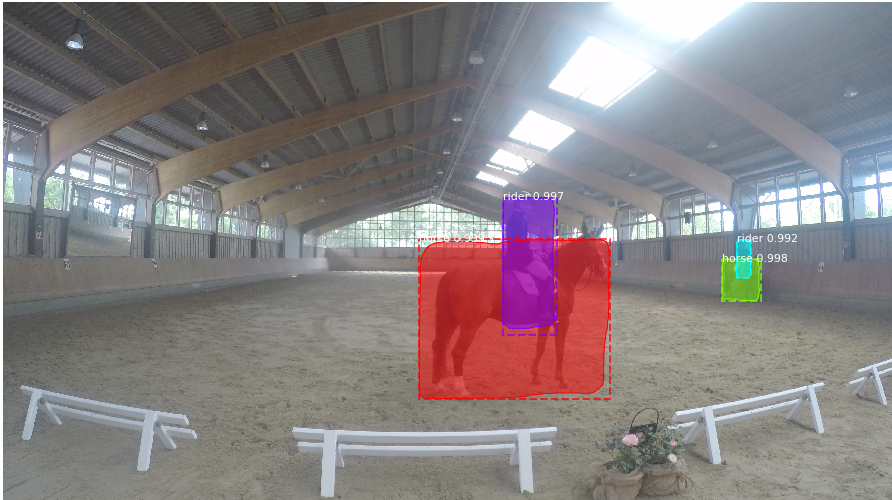
\includegraphics[height=4cm,trim={12cm 0 3cm 0},clip]{./img/IndoorMaske.png}
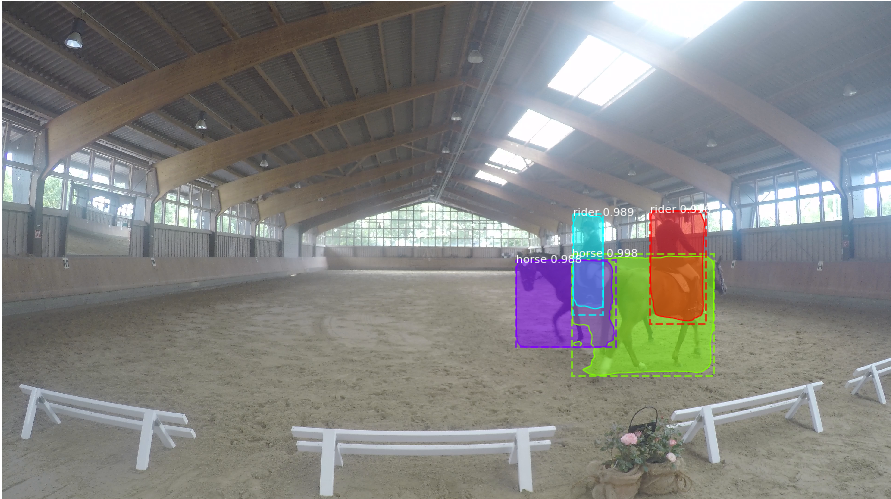
\includegraphics[height=4cm,trim={15cm 0 0 0},clip]{./img/IndoorMaske2.png}
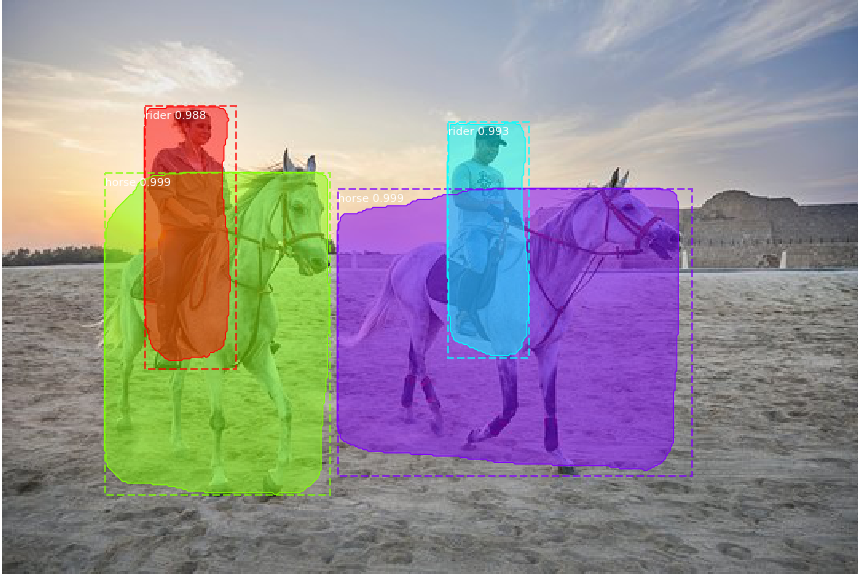
\includegraphics[height=4cm,trim={1cm 0 3cm 0},clip]{./img/OutdoorMaske.png}
\caption{Segmentierung von Reiter und Pferd nach dem Training der zweiten Phase}
\label{fig:SegmentierungPhase2}
\end{figure}

Zur vielfältigen Nutzung des erstellten Detektors, haben wir das Training mit weiteren gelabelten Bilddaten ermöglicht, um den Detektor auch in anderen Hallen zuverlässiger verwenden zu können. Dazu werden die Bilder eines Ordners nacheinander angezeigt, wobei die detektierten Pferde und Reiter mit farbigen Bounding Boxen eingezeichnet werden. Anhand dieser Boxen kann der Nutzer entscheiden, ob die Daten geeignet sind, sodass die akzeptierten Bilder und deren Boxen wie in der Ordnerstruktur von \ref{fig:folderstructure} wiederum abgespeichert werden, um den Detektor damit weiter zu trainieren.

\subsection*{Extraktion der Rois}

Mithilfe von OpenCV werden alle Frames des Eingabevideos einzeln durchlaufen und der zuvor trainierte Detektor auf jedes einzeln angewandt. Dadurch haben wir pro Frame alle erkannten Reiter und Pferde mittels Bounding Boxen abgespeichert und anhand dieser weiter die Rois berechnet, da unser Fokus aus Zeitgründen noch nicht auf Erkennung von Reiterpaaren lag. Wir verfolgten hier den Ansatz zunächst alle Reiter und Pferde in den Rois abzubilden und erst in der dritten Phase zu selektieren um auf ein einzelnes Paar zu fokussieren. Dieser Modus kann weiterhin gut für Aufwärmphasen der Reitturniere genutzt werden, bei denen mehrere Reiterpaare auf dem Turnierplatz sind. Die Umsetzung ist als austauschbarer Filter konzipiert, der eine Gesamt-Bounding-Box anhand der maximalen und minimalen Eckpunkte aller detektierten Bounding-Boxen bestimmt.
Ausgehend von der Gesamt-Bounding-Box müssen für die Erstellung erster Videos noch nötige Sonderfälle beachtet werden. So wird der Zoom unter 480 Pixel verhindert, um eine gute Bildqualität zu ermöglichen. Die längere Seite der Bounding-Box ist ausschlaggebend für die Berechnung der passenden Ratio des Bildausschnittes, sodass dann die optimalen  Eckpunkte berechnet werden können. Wichtig ist es noch die Ränder eines Frames zu berücksichtigen und die Ratio entsprechend zu korrigieren.
Im letzten Schritt werden die Rois mithilfe der kalkulierten Gesamtbox aus jedem Frame ausgeschnitten  . Nachdem alle Frames auf die gleiche Größe gebracht werden, was durch die gleiche Ratio aller Frames keine Verzerrung zur Folge hat, werden die Frames mit OpenCV in ein Ausgabevideo geschrieben.

\todo{Reiterpaare}
\subsection*{Reiterpaar Erkennung}



\section{Phase 3}
\subsection*{Weiterentwicklung des Detektors}

\begin{figure}[b]
\centering
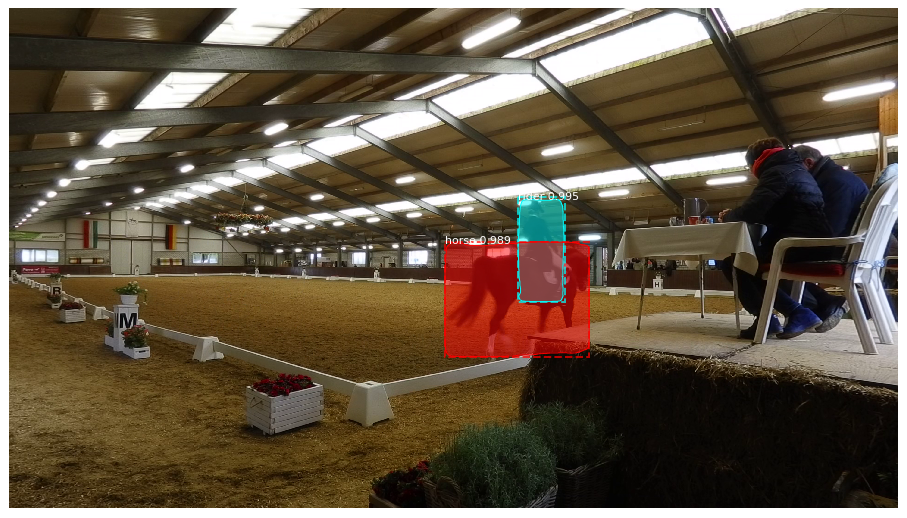
\includegraphics[height=4cm,trim={6cm 0 6cm 0},clip]{./img/IndoorMask6.png}
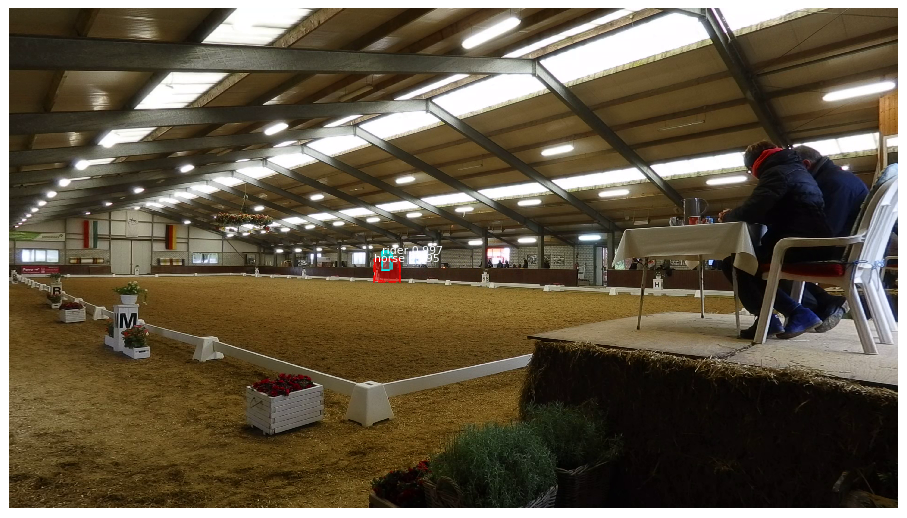
\includegraphics[height=4cm,trim={6cm 0 6cm 0},clip]{./img/IndoorMask3.png}
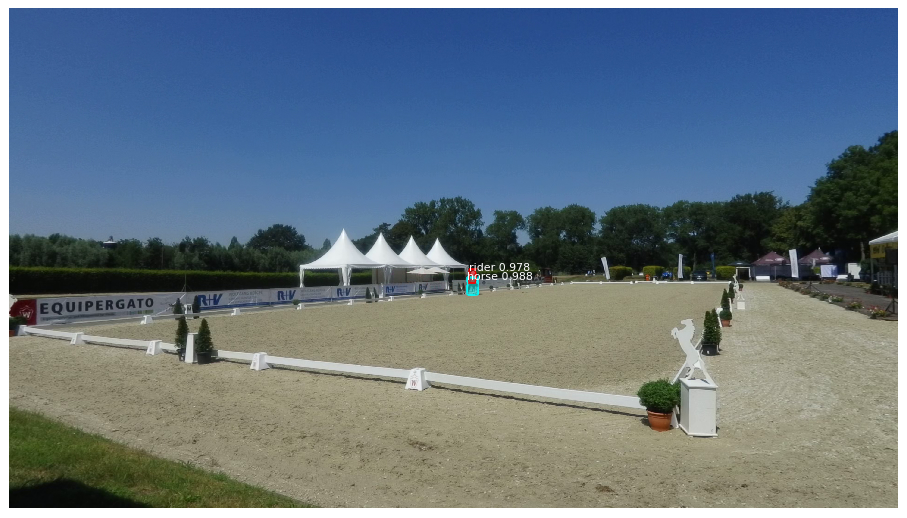
\includegraphics[height=4cm,trim={6cm 0 6cm 0},clip]{./img/OutdoorMask2.png}
\caption{Segmentierung von Reiter und Pferd nach dem Training der zweiten Phase}
\label{fig:SegmentierungPhase3}
\end{figure}

Mit Beginn der dritten Phase wurden weitere Reitvideos zur Verfügung gestellt, welche in verschiedenen Hallen sowie im Außenbereich gefilmt wurden. Der erste Test mit dem Detektor der zweiten Phase verlief nicht sonderlich zufriedenstellend, wodurch wir mehrere Probleme identifizieren konnten. Zum einen wurden nicht alle Reiter und Pferde, die weit entfernt von der Kamera waren, korrekt detektiert. Dieses Ergebnis war aufgrund des zuvor recht einseitigen Trainings nicht verwunderlich, da sich die Hintergründe, Reiter und Pferde unterschieden. Zum anderen wurden auch viele sitzende Personen als Reiter identifiziert und einige Gegenstände wie beispielsweise Pflanzen als fehlerhaft erkannt. Nachdem wir jedoch ungefähr 100 weitere Frames pro neuer Umgebung ausgewählt und damit den Detektor weiter trainiert hatten, wurden ein Großteil der Fehler beseitigt (siehe \ref{fig:SegmentierungPhase3}). Durch die Erweiterung des Detektors ist dieser nun auch in der Lage unterschiedlich gekleidete Reiter und Pferde mit abweichende Fellfarben zuverlässiger zu detektieren.


\subsection*{Benutzeroberfläche}

Im Hinblick auf die Kundengruppe haben wir das Kennzeichnung weiterer Bilddaten und die Konvertierung eines Videos für autonome Kameraführung in eine GUI eingebunden. Die GUI wurde mit PyQt5 erstellt und das Standardaussehen durch Einbinden eines Stylesheets modifiziert. Mit dieser minimalen Benutzeroberfläche kann der Nutzer nun zunächst auswählen ob weitere Daten gelabelt werden sollen oder ein Video umgewandelt werden soll. Bei der Auswahl weiter Bilddaten können sowohl Ordner mit Bildern als auch Videos mithilfe extrahierter Frames verwendet werden. Dazu kann der Nutzer pro Bild entscheiden ob die eingezeichnete Detektion gut genug ist diese akzeptieren oder ablehnen und im Anschluss den Detektor damit weiter trainieren. Für die Umwandlung eines Videos wird nach Auswahl der Datei und der Auflösung des Ausgabeformates ein Video unseres Smart Camera Operators erstellt.
\todo{Screenshots Gui Start, Gui Labelling, Gui Convert}


\subsection*{Videoqualität}
\subsubsection*{Performance}
Da der Fokus unserer Gruppe auf der Genauigkeit des Detektors liegt, haben wir nur einige grundlegende Verbesserungen der Performance vorgenommen, welche dem nicht entgegenwirken. 
Im ersten Schritt wir dazu anhand der Auflösung des Eingabevideos entschieden, ob die Frames vor der Detektion verkleinert werden sollten. Dies war bei den aufgenommenen Videos mit 4k Auflösung sinnvolle, da Mask Rcnn auch mit einfacher HD Auflösungen ähnlich gute Ergebnisse liefert. Somit konnte der Zeitaufwand der Detektion von ca. 0.81  auf ca. 0.48 Sekunden pro Detektion verbessert werden. Anschließend müssen die detektierten Boxen wieder entsprechend hochskaliert werden um mit den Ursprungsbilder übereinzustimmen.

Als weitere Verbesserung haben wir den Einsatz von Ausgleichsgeraden und Ausgleichskurven getestet. Als Ansatz haben wir den Gedankengang verfolgt, nicht für jeden Frame Detektionen durchzuführen, sonder nur für jeden n-ten Frame, wodurch die Anwendung beschleunigt würde. 
In beiden Fällen haben wir mithilfe von "numpy.polyfit" die Berechnungen anhand der letzten 10 Detektionen erstellt. Die Ergebnisse für die Ausgleichsgerade stellten sich zwar performancemäßig als sehr positiv dar, jedoch ging die Videoqualität stark zurück. Das Ausgabevideo wies aufgrund der Ausgleichsgeraden sehr regelmäßige gerade Kameratranslationen auf, die die Gesamtqualität verminderten.
Als nächstes nutzten wir statt der Geraden Ausgleichskurven, wobei sich bereits Kurven vom Grad 2 oder 3 ausreichend gut eigneten. Während dadurch die vorherigen Makel im Ausgabevideo gelöst wurden, stellte sich nur sehr geringfügiger bis gar kein Performacevorteil heraus. Aufgrund dessen wurden beide Versuche die Anzahl der Detektionen zu verringern verworfen und aus Zeitgründen nicht weiter verfolgt.




\subsubsection*{Sprünge/Verschwinden}
\subsubsection*{Verdecken}

\subsection*{Reiterpaarerkennung}
Aus der Detektion erhalten wir eine Menge aus RoIs(bounding boxen).
Jede Box umrandet einen Mensch oder ein Pferd. Diese Menge aus RoIs wird gefiltert. Wir möchten nur Reiterpaare haben. Ein Reiterpaar ist ein Mensch sehr nah an oder auf einem Pferd.

Eine Box ist ein Rechteck. Wir können also berechnen, wie groß der Flächeninhalt der überlappenden Rechtecke ist. Flächeninhalt gleich Null bedeutet, sie überlappen sich überhaupt nicht.
Dadurch ist es nicht nur möglich zu berechnen, ob eine Pferd nah an einem Menschen ist - sondern auch wie nah. Es kann ein Threshold gewählt werden, der die Größe des Flächeninhalts prüft. Beispielsweise hätte ein Mensch \emph{auf} einem Pferd einen größeren Flächeninhalt als ein Mensch \emph{neben} einem Pferd. Je nach Wunsch kann das also angepasst werden bei uns.


Wenn eine Mensch-RoI also eine Pferd-RoI überlappt, zeichnen wir um beide eine Reiterpaar-RoI.

\subsection*{Glättung}
Um die Folge der RoIs zu glätten, damit sich nach dem Zuschneiden ein sanftes Seherlebnis für den Zuschauer bietet, haben wir verschiedene Verfahren ausprobiert.


Das effektivste, effizienteste und gleichzeitig das einfachste Verfahren, das wir hatten war ein eindimensionaler Gaußfilter.
Wir haben eine Folge aus RoIs.
Jede RoI hat 4 Attribute - die Koordinaten $(x1,y1), (x2,y2)$ des Rechtecks.
Wir schieben über alle $x1, y1, x2, y2$ aller RoIs einen 1d-Gaußfilter mit $\sigma=5$ drüber.
Wir schieben also insgesamt 4 Mal einen Filter über die RoIs für jedes der 4 Attribute.


Eine weitere Möglichkeit wäre es gewesen, die Richtungsänderungen zu erkennen/berechnen und dann einfach die RoIs linear von einer Richtungsänderung zur nächsten wandern zu lassen. Das wäre auch für die Echtzeit-Anwendung nötig gewesen, da hier die Kamera ja rotieren muss bei Richtungsänderung.
Die Richtungsänderungen lassen sich mit \emph{optical flow} berechnen.
Wir haben aber auch eine für unseren Anwendungsfall effizientere Möglichkeit gefunden, die aber aus Platzgründen und weil sie sowieso nicht implementiert wurde hier nicht weiter thematisiert wird.


\chapter{Ergebnisauswertung}
\label{ch:ergebnis}

Qualitative Auswertung:

•	Diskussion Zielerreichung

•	Untersuchung der Bedienung


•	Empfehlung noch nicht implementierter Funktionen

\vspace{1cm}

Bugs:

•	Prototyp

•	fehlender Praxistest

•	bisher nur Grundfunktionen

\vspace{1cm}

Verbesserungen:

•	Performance für Live Übertragung

•	Model Training erweitern

•	Festlegung welchem Reiterpaar situationsbedingt gefolgt werden soll

•	Bildentzerrung?


\vspace{1cm}
Zusammenfassung der Beobachtungen
	
	
•	Einstufung der Fehler und ihre Wichtigkeit

•	Fehlertoleranz

•	Ursachenanalyse
	
•	Verbesserungsvorschläge
	
•	Interssenskonflike(Performance und Zeitaufwand)
	
•	Beurteilung der Resourcen (Zeit, Vorwissen, erworbene Kenntnisse )

•	Effektivität

•	Effizienz

•	Zufriedenstellung/Akzeptanz

•	Aufgabenangemessenheit

•	Erlernbarkeit

•	Erwartungskonformität



\section{Planung}
Die vorgegebenen Phasen aus der Aufgabenstellung dieses Projektes stellten sich als sehr hilfreich für ein sinnvolles schrittweises Vorgehen und dessen Umsetzung heraus, besonders im Hinblick auf fehlendes Vorwissen aller Gruppenmitglieder in der Thematik Maschine Learning. Während die erste Phase problemlos ablief, gestaltete sich der praktische Einstieg in Phase zwei dagegen relativ langwierig bis wir einen ersten Prototypen unseres Detektors erstellen konnten. Als Folge dessen war es uns nicht vollständig möglich das Ziel eines Reiterpaardetektors bereits in Phase 2 fertigzustellen, da dieser an einigen Stellen noch Fehler aufwies, welche jedoch direkt zu Beginn der dritten Phase behoben wurden. Ebenfalls sollte in der zweiten Phase das Labelling weiterer Daten umgesetzt werden, wobei die entsprechend vereinfachte Benutzung dieses Zieles erst mithilfe der GUI in Phase drei hinzugefügt wurde. Diese zeitlichen Verschiebungen konnten jedoch in mit effizienter Aufgabenteilung gut bewältigt werden und stellten kein Hindernis für die letzte Phase dar.
Durch die recht allgemeine Formulierung der Ziele in Phase drei, die einen Fokus auf robustes und flüssiges Tracking, haben wir die daraus abgeleiteten Gruppenziele in den Vordergrund gestellt. Obwohl einige Konzepte, die aus Effizienz- oder Performancegründen verworfen wurden, erprobt wurden, konnten die Projektziele eingehalten werden. 

\section{Umsetzung und Zielerreichung}

\subsection*{Umsetzung GUI}
•	Genereller Überblick

•	Spezielle Bedienelemente

•	Ausführung vorgegebener Handlungsabläufe

•	Leichte Erlernbarkeit


\subsection*{Umsetzung Detektor}

\subsection*{Umsetzung Tracker}

\section{Verbesserungen}



\chapter{Schlussfolgerung und Ausblick}
\label{ch:zusammenfassung}


Ausblick:

•	Einsatzmöglichkeiten für Turniere und Trainingsstunden

\begin{appendices}
\chapter{Anhang}
\label{ch:anhang}

Videoverweise

\end{appendices}

\backmatter

% Literaturverzeichnis
\bibliographystyle{unsrtdin}

\bibliography{Quellen}




% Eidesstattliche Erklärung
%\include{chapter/EidesstattlicheErklaerung}

\end{document}
